
\documentclass[9pt]{beamer}

\usepackage{inputenc}
\usepackage[T1]{fontenc}
\usepackage{textcomp}
\usepackage{amsmath}
\usepackage{amsthm}
\usepackage{amssymb}
\usepackage{euler}
\usepackage{fontspec}
\usepackage{minted}
\usepackage{graphicx}
\usepackage{fancyvrb}
\usepackage{bbold}

\usetheme[titleformat=smallcaps,block=fill]{metropolis}

%\renewcommand{\rmdefault}{eulervm}

%\usefonttheme{professionalfonts}
\setmonofont[Scale=0.8]{Menlo}
%\usefonttheme[onlymath]{serif}

\usemintedstyle{xcode}

\setbeamertemplate{blocks}[rounded]

%Information to be included in the title page:
\title{PhD defense}
\author{{\small candidate:} Massimo Nocentini \hfill {\small advisor:} prof. Donatella Merlini }
\institute{University of Florence, Italy.}
%\vfill
\includegraphics[width=\textwidth]{logo}}
\date{\today}

\begin{document}

\frame{\titlepage}


\begin{frame}[fragile]
\frametitle{This talk needs no title}
\begin{Verbatim}
$ whoami
Massimo Nocentini
PhD candidate @ University of Florence
Mathematician (algebraic combinatorics, formal methods for algs)
Programmer (automated reasoning, logics and symbolic comp)
https://github.com/massimo-nocentini (50 public repos)
\end{Verbatim}

\begin{block}{}
I'm here to defend my way of doing \textit{combinatorics}. \\
My methodology is deeply connected to \textit{recursion schemata}.

Their combination shows that the study of the former entails the study of the
latter and the study of the latter entails the study of the former,
recursively.
\end{block}

\end{frame}

\begin{frame}[fragile]
\frametitle{Backgrounds}
According to Wilf, a
generating function is a clothesline on which we hang up a sequence of
numbers for display; btw, $C(t)$ shows the Catalan numbers,
\begin{displaymath}
 C(t) = \frac{1-\sqrt{1-4t}}{2t} = 1 + t + 2t + 5t^{2} + 14t^{3} + 42t^{4} + O(t^{5}).
\end{displaymath}
A Riordan array is a l.t.i. matrix denoted by a pair $(d(t), h(t))$ s.t. $h(0)=0$, 
\begin{itemize}
\item whose $k$-th column $\textbf{c}_{k}$ is recursively defined as 
\begin{displaymath}
 \textbf{c}_{k+1} =h(t) \textbf{c}_{k} \quad\text{provided that}\quad \textbf{c}_{k} = d(t)h(t)^{k} ;
\end{displaymath}
\item whose coefficients are recursively defined as
\begin{displaymath}
 d_{n+1, k+1} = a_{0}d_{n, k} + a_{1}d_{n, k+1} + a_{2}d_{n, k+2} + \ldots + a_{j}d_{n, k + j}, \quad k + j = n
\end{displaymath}
where $A(t) = \sum_{j\in\mathbb{N}}{a_{j}t^{j}}$ satisfies $h(t) = t\,A(h(t))$; finally,
\item the set $\mathcal{R}$ of Riordan arrays with the
operation $(d(t), h(t))\cdot(g(t), f(t)) = (d(t)g(h(t)), f(h(t)))$
makes $(\mathcal{R}, \cdot)$ a group.
\end{itemize}


\end{frame}


\section{Binary words and algebraic gfs}

\begin{frame}[fragile]
\frametitle{Enumeration of binary words avoiding a given pattern}

Languages $\mathfrak{L}^{[\mathfrak{p}]}\subset \{0,1\}^*$ of binary words $w$
avoiding a \textit{Riordan pattern} $\mathfrak{p}$ are enumerated,
wrt $1$-bits and $0$-bits, by
$$F^{[\mathfrak{p}]}(x,y)
=\genfrac{}{}{1pt}{0}{C^{[\mathfrak{p}]}(x,y)}{(1-x-y)C^{[\mathfrak{p}]}(x,y)
+x^{n_1^{[\mathfrak{p}]}}y^{n_0^{[\mathfrak{p}]}}}$$
Let $R_{n,k}^{[\mathfrak{p}]}$ be the number of words avoiding $\mathfrak{p}$
and having $n$ $1$-bits  and $n-k$  $0$-bits, formally
${\mathcal{F}_{n,k}^{[\mathfrak{p}]}} = {\mathcal{R}_{n,
n-k}^{[\bar{\mathfrak{p}]}}}$; moreover, let
$\mathcal{R}^{[\mathfrak{p}]}=\left(R_{n,k}^{[\mathfrak{p}]}\right)_{n,k\in\mathbb{N}}$
be the enclosing matrix and ${\cal{R}^{[\mathfrak{p}]}}$ is a
\textit{Riordan array} if and only if  $\mathfrak{p}$ is a Riordan pattern.
\vfill
\noindent\rule{\textwidth}{0.1pt}
{\footnotesize
Merlini \& Nocentini. \textit{Algebraic Generating Functions for Languages
Avoiding Riordan Patterns}.  Journal of Integer Sequences, 2018.}
\end{frame}

\begin{frame}[fragile]
\frametitle{Enumeration of binary words avoiding a Riordan pattern}

Let $\mathfrak{p}$ be a Riordan pattern
such that $n_1^{[\mathfrak{p}]}-n_0^{[\mathfrak{p}]}=1$, then
$\mathcal{R}^{\left[\mathfrak{p}\right]}$ is defined by
$$d^{[\mathfrak{p}]}(t)={C^{[\mathfrak{p}]}(t)
\over \sqrt{C^{[\mathfrak{p}]}(t)^2-4tC^{[\mathfrak{p}]}(t)(C^{[\mathfrak{p}]}(t)-t^{n_0^{[\mathfrak{p}]}})}}\quad\text{and}$$
$$h^{[\mathfrak{p}]}(t)={C^{[\mathfrak{p}]}(t) -\sqrt{C^{[\mathfrak{p}]}(t)^2-4tC^{[\mathfrak{p}]}(t)(C^{[\mathfrak{p}]}(t)-t^{n_0^{[\mathfrak{p}]}})}
\over 2 C^{[\mathfrak{p}]}(t)},$$
where $C^{[\mathfrak{p}]}(t)=C^{[\mathfrak{p}]}(\sqrt{t},\sqrt{t})$
and the \textit{bivariate auto-correlation polynomial}
\begin{displaymath}
C^{[\mathfrak{p}]}(x,y)=C^{[\mathfrak{\bar{p}}]}(y,x)=\sum_{i=0}^{\lfloor(h-1)/2\rfloor}c_{2i}x^iy^i,
\end{displaymath}
is defined wrt $c_i=[\![p_0p_1\cdots p_{h-1-i}=p_{i}p_{i+1}\cdots p_{h-1}]\!]$;
moreover, similar functions can be defined for cases
$n_1^{[\mathfrak{p}]}-n_0^{[\mathfrak{p}]}=0$ and
$n_1^{[\mathfrak{p}]}-n_0^{[\mathfrak{p}]}=-1$.

\vfill
\noindent\rule{\textwidth}{0.1pt}
{\footnotesize
Merlini \& Nocentini. \textit{Algebraic Generating Functions for Languages
Avoiding Riordan Patterns}.  Journal of Integer Sequences, 2018.}
\end{frame}

\begin{frame}[fragile]
\frametitle{Enumeration of constrained binary words avoiding a Riordan pattern}

Add the constraint $|w|_0\leq |w|_1$, for any $w\in \mathfrak{L}^{[\mathfrak{p}]}$.
\begin{itemize}
\item $S^{[\mathfrak{p}]}(t)$ enumerates $\left\lbrace w\in \lbrace 0,1 \rbrace^{*}:
|w|_0\leq |w|_1\right\rbrace$ avoiding $\mathfrak{p}$\newline according to
\textit{the number of $1$-bits},
$$S^{[\mathfrak{p}]}(t)={2C^{[\mathfrak{p}]}(t) \over \sqrt{Q(t)}\left(\sqrt{C^{[\mathfrak{p}]}(t)}+ \sqrt{Q(t)} \right)} $$
    where $Q(t)={(1-4t)C^{[\mathfrak{p}]}(t)^2+4t^{n_1^{[\mathfrak{p}]}}}.$
\item $L^{[\mathfrak{p}]}(t)$ enumerates $\left\lbrace w\in \lbrace 0,1 \rbrace^{*}:
|w|_0\leq |w|_1\right\rbrace$ avoiding $\mathfrak{p}$\newline according to
\textit{the word length},
$$L^{[\mathfrak{p}]}(t)= {2tC^{[\mathfrak{p}]}(t^2)^2 \over \sqrt{Q(t)}\left((2t-1)C(t^2)+ \sqrt{ Q(t) } \right)}$$
where $Q(t)=C^{[\mathfrak{p}]}(t^2)\left( (1-4t^2)C^{[\mathfrak{p}]}(t^2)+4t^{2n_1^{[\mathfrak{p}]}}\right).$
\end{itemize}
\vfill
\noindent\rule{\textwidth}{0.1pt}
{\footnotesize
Merlini \& Nocentini. \textit{Algebraic Generating Functions for Languages
Avoiding Riordan Patterns}.  Journal of Integer Sequences, 2018.}
\end{frame}


\section{Matrices functions}

\begin{frame}[fragile]
\frametitle{Functions of Riordan matrices}
\begin{columns}
    \begin{column}{0.6\textwidth}
        \begin{displaymath}
        \footnotesize
        %\mathcal{P}_{8}=\left[\begin{matrix}1 &   &   &   &   &   &   &  \\1 & 1 &   &   &   &   &   &  \\1 & 2 & 1 &   &   &   &   &  \\1 & 3 & 3 & 1 &   &   &   &  \\1 & 4 & 6 & 4 & 1 &   &   &  \\1 & 5 & 10 & 10 & 5 & 1 &   &  \\1 & 6 & 15 & 20 & 15 & 6 & 1 &  \\1 & 7 & 21 & 35 & 35 & 21 & 7 & 1\end{matrix}\right]
        \mathcal{C}_{8}=\left[\begin{matrix}1 &   &   &   &   &   &   &  \\1 & 1 &   &   &   &   &   &  \\2 & 2 & 1 &   &   &   &   &  \\5 & 5 & 3 & 1 &   &   &   &  \\14 & 14 & 9 & 4 & 1 &   &   &  \\42 & 42 & 28 & 14 & 5 & 1 &   &  \\132 & 132 & 90 & 48 & 20 & 6 & 1 &  \\429 & 429 & 297 & 165 & 75 & 27 & 7 & 1\end{matrix}\right]
        \end{displaymath}
        \begin{displaymath}
        \footnotesize
        e^{\mathcal{C}_{8}} = e \left[\begin{matrix}1 &   &   &   &   &   &   &  \\1 & 1 &   &   &   &   &   &  \\3 & 2 & 1 &   &   &   &   &  \\\frac{23}{2} & 8 & 3 & 1 &   &   &   &  \\\frac{154}{3} & 37 & 15 & 4 & 1 &   &   &  \\\frac{1 27}{4} & \frac{572}{3} & \frac{163}{2} & 24 & 5 & 1 &   &  \\\frac{7 46}{5} & \frac{6439}{6} & 478 & 15  & 35 & 6 & 1 &  \\\frac{5 2481}{6 } & \frac{39 899}{6 } & \frac{12  5}{4} & \frac{2965}{3} & \frac{495}{2} & 48 & 7 & 1\end{matrix}\right]
        \end{displaymath}
    \end{column}
    \begin{column}{0.4\textwidth}
    Lift the scalar function $$f: \mathbb{R} \rightarrow \mathbb{R}$$
    to the matrix function
    $$\hat{f}: \mathbb{R}^{m\times m} \rightarrow \mathbb{R}^{m\times m}$$
    where $m\in\mathbb{N}$, provided that
    \begin{displaymath}
        \left. \frac{\partial^{(j)}{f}}{\partial{z}^{j}} \right|_{z=\lambda_{i}},\,
        \begin{array}{l}
            i\in \lbrace 1, \ldots, \nu \rbrace \\
            j \in \lbrace 0, \ldots, m_{i}-1 \rbrace
        \end{array},
    \end{displaymath}
    exists, for each eigenvalue $\lambda_{i}$.
    \end{column}
\end{columns}
\vfill
\noindent\rule{\textwidth}{0.1pt}
{\footnotesize
Merlini \& Nocentini. \textit{Functions and Jordan Canonical Forms of Riordan
matrices}. \newline Linear Algebra and its Applications, Volume 565, Pages 177-207, 2019.}
\end{frame}

\begin{frame}[fragile]
\frametitle{Functions of Riordan matrices}
\begin{displaymath}
\footnotesize
    \mathcal{P}_{8}=\left[\begin{matrix}1 &   &   &   &   &   &   &  \\1 & 1 &   &   &   &   &   &  \\1 & 2 & 1 &   &   &   &   &  \\1 & 3 & 3 & 1 &   &   &   &  \\1 & 4 & 6 & 4 & 1 &   &   &  \\1 & 5 & 10 & 10 & 5 & 1 &   &  \\1 & 6 & 15 & 20 & 15 & 6 & 1 &  \\1 & 7 & 21 & 35 & 35 & 21 & 7 & 1\end{matrix}\right]
    \quad
    \sqrt[3]{\mathcal{P}_{8}}= \left[\begin{matrix}1 &  &  &  &  &  &  & \\\frac{1}{3} & 1 &  &  &  &  &  & \\\frac{1}{9} & \frac{2}{3} & 1 &  &  &  &  & \\\frac{1}{27} & \frac{1}{3} & 1 & 1 &  &  &  & \\\frac{1}{81} & \frac{4}{27} & \frac{2}{3} & \frac{4}{3} & 1 &  &  & \\\frac{1}{243} & \frac{5}{81} & \frac{10}{27} & \frac{10}{9} & \frac{5}{3} & 1 &  & \\\frac{1}{729} & \frac{2}{81} & \frac{5}{27} & \frac{20}{27} & \frac{5}{3} & 2 & 1 & \\\frac{1}{2187} & \frac{7}{729} & \frac{7}{81} & \frac{35}{81} & \frac{35}{27} & \frac{7}{3} & \frac{7}{3} & 1\end{matrix}\right]
\end{displaymath}

such that %$\sqrt{\mathcal{P}_8} \cdot \sqrt{\mathcal{P}_8} =\mathcal{P}_8$ and
$\sqrt[3]{\mathcal{P}_8} \cdot \sqrt[3]{\mathcal{P}_8} \cdot
\sqrt[3]{\mathcal{P}_8} =\mathcal{P}_8$ and
$L_{8}\left({e^{\mathcal{C}_{8}}}\right) = \mathcal{C}_{8}$, where polynomial
\begin{displaymath}
{L_{ 8 }}{\left (z \right )} = \frac{z^{7}}{7 e^{7}} - \frac{7 z^{6}}{6 e^{6}} + \frac{21 z^{5}}{5 e^{5}} - \frac{35 z^{4}}{4 e^{4}} + \frac{35 z^{3}}{3 e^{3}} - \frac{21 z^{2}}{2 e^{2}} + \frac{7 z}{e} - \frac{223}{140}
\end{displaymath}
interpolates the $log$ function; moreover, the classic identity
$$sin(\mathcal{P}_8)\cdot sin(\mathcal{P}_8)+
cos(\mathcal{P}_8)\cdot cos(\mathcal{P}_8)=I_{8},$$
where $I$ is the identity matrix, holds as well.
\vfill
\noindent\rule{\textwidth}{0.1pt}
{\footnotesize
Merlini \& Nocentini. \textit{Functions and Jordan Canonical Forms of Riordan
matrices}. \newline Linear Algebra and its Applications, Volume 565, Pages 177-207, 2019.}
\end{frame}

\begin{frame}[fragile]
\frametitle{Functions of Riordan matrices}
Generalized Lagrange bases and Hermite interpolating polys
\begin{columns}
    \begin{column}{0.5\textwidth}
        \begin{displaymath}
        \footnotesize
        \left. \frac{\partial^{(r-1)}{\Phi_{i,j}}}{\partial{z}^{r-1}} \right|_{z=\lambda_{l}} = \delta_{i,l}\delta_{j,r},
        \,
        \begin{array}{l}
            l\in \lbrace 1, \ldots, \nu \rbrace \\
            r \in \lbrace 1, \ldots, m_{l} \rbrace
        \end{array}
        \end{displaymath}
        \begin{displaymath}
        \footnotesize
        g(z) = \sum_{i=1}^{\nu}{\sum_{j=1}^{m_{i}}{ \left.
        \frac{\partial^{(j-1)}{f}}{\partial{z}^{j-1}} \right|_{z=\lambda_{i}}\Phi_{i,j}(z) }}
        \end{displaymath}
    \end{column}
    \vrule{}
    \begin{column}{0.5\textwidth}
        \begin{displaymath}
        \footnotesize
          \Phi_{1,j}(z) = \frac{\left(z-\lambda_{1}\right)^{j-1}}{(j-1)!},
          \, j\in \lbrace 1,\ldots, m_{1} \rbrace
        \end{displaymath}
        \begin{displaymath}
        \footnotesize
        g_{m}(z) = {\sum_{j=1}^{m}{ \left.
        \frac{\partial^{(j-1)}{f}}{\partial{z}^{j-1}} \right|_{z=\lambda_{1}}}}
        \frac{\left(z-\lambda_{1}\right)^{j-1}}{(j-1)!}
        \end{displaymath}
    \end{column}
\end{columns}
for \textit{arbitrary} and \textit{Riordan} matrices, respectively.
We study functions
\begin{displaymath}
\begin{split}
f(z)&=z^{r},\,{f(z)=\frac{1}{z}},\,{f(z)=\sqrt{z}},\,{f(z)=e^{\alpha z}},\\
f(z)&=log\,{z},\,f(z)=sin\,{z}\quad\text{and}\quad f(z)=cos\,{z}
\end{split}
\end{displaymath}
and their applications to Riordan matrices $\mathcal{P}_{8}$, $\mathcal{C}_{8}$
and $\mathcal{S}_{8}$.
\vfill
\noindent\rule{\textwidth}{0.1pt}
{\footnotesize
Merlini \& Nocentini. \textit{Functions and Jordan Canonical Forms of Riordan
matrices}. \newline Linear Algebra and its Applications, Volume 565, Pages 177-207, 2019.}
\end{frame}

\begin{frame}[fragile]
\frametitle{Functions of Riordan matrices}
\begin{columns}
    \begin{column}{0.35\textwidth}
        \begin{displaymath}
        \begin{split}
          P_{m}(z) &= \sum_{j=0}^{m-1}{\binom{r}{j}}{(z-1)^{j} }\\
          I_{m}(z) &= \sum_{j=0}^{m-1}{(-1)^{j}\,\left(z-1\right)^{j}}\\
          R_{m}(z) &= \sum_{j=0}^{m-1}{{\frac{1}{2} \choose j}\left(z-1\right)^{j}}\\
          E_{m}(z) &= e^{\alpha} \sum_{j=0}^{m-1}{\frac{\alpha^{j}}{j!}\left(z-1\right)^{j}}\\
          L_{m}(z) &= \sum_{j=1}^{m-1}{\frac{(-1)^{j-1}}{j}{\left(z-1\right)^{j} }}\\
        \end{split}
        \end{displaymath}
    \end{column}
    \vrule{}
    \begin{column}{0.65\textwidth}
        \begin{displaymath}
        \footnotesize
        \begin{split}
          S_{m}(z)  &= sin\,{1}\,\sum_{k=0}^{2\,\left\lceil \frac{m}{2} \right\rceil-2}{\left(\sum_{j=\left\lceil \frac{k}{2}\right\rceil}^{\left\lceil \frac{m}{2} \right\rceil -1}{\frac{(-1)^{3j}}{(2j)!}{2j\choose k}}\right) {(-z)^{k}}}\\
                    &+ cos\,{1}\,\sum_{k=0}^{2\,\left\lfloor \frac{m}{2} \right\rfloor-1}{\left(\sum_{j=\left\lfloor \frac{k}{2}\right\rfloor}^{\left\lfloor \frac{m}{2} \right\rfloor -1}{\frac{(-1)^{3j+1}}{(2j + 1)!} {2j+1\choose k}}\right){(-z)^{k}}}\\
          C_{m}(z)  &= cos\,{1}\,\sum_{k=0}^{2\,\left\lceil \frac{m}{2} \right\rceil-2}{\left(\sum_{j=\left\lceil \frac{k}{2}\right\rceil}^{\left\lceil \frac{m}{2} \right\rceil -1}{\frac{(-1)^{3j}}{(2j)!}{2j\choose k}}\right) {(-z)^{k}}}\\
                    &+ sin\,{1}\,\sum_{k=0}^{2\,\left\lfloor \frac{m}{2} \right\rfloor-1}{\left(\sum_{j=\left\lfloor \frac{k}{2}\right\rfloor}^{\left\lfloor \frac{m}{2} \right\rfloor -1}{\frac{(-1)^{3j+2}}{(2j + 1)!} {2j+1\choose k}}\right){(-z)^{k}}}\\
        \end{split}
        \end{displaymath}
    \end{column}
\end{columns}
where $c\cdot(d_{n,k})_{n,k\in\mathbb{N}} = (c\cdot d_{n,k})_{n,k\in\mathbb{N}}$
and $c\in\mathbb{R}$.
\vfill
\noindent\rule{\textwidth}{0.1pt}
{\footnotesize
Merlini \& Nocentini. \textit{Functions and Jordan Canonical Forms of Riordan
matrices}. \newline Linear Algebra and its Applications, Volume 565, Pages 177-207, 2019.}
\end{frame}

\begin{frame}[fragile]
\frametitle{Functions of Riordan matrices}

    Let $r\in\mathbb{Q}$; matrices $\mathcal{P}_{8}^{r}, \mathcal{S}_{8},
    log{\mathcal{P}_{8}}$ and $\sqrt{\mathcal{S}_{8}}$ are defined as
    \begin{displaymath}
    \footnotesize
      \left[\begin{matrix}1 &   &   &   &   &   &   &  \\r & 1 &   &   &   &   &   &  \\r^{2} & 2 r & 1 &   &   &   &   &  \\r^{3} & 3 r^{2} & 3 r & 1 &   &   &   &  \\r^{4} & 4 r^{3} & 6 r^{2} & 4 r & 1 &   &   &  \\r^{5} & 5 r^{4} & 10 r^{3} & 10 r^{2} & 5 r & 1 &   &  \\r^{6} & 6 r^{5} & 15 r^{4} & 20 r^{3} & 15 r^{2} & 6 r & 1 &  \\r^{7} & 7 r^{6} & 21 r^{5} & 35 r^{4} & 35 r^{3} & 21 r^{2} & 7 r & 1\end{matrix}\right],\,
      \left[\begin{matrix}1 &  &  &  &  &  &  & \\1 & 1 &  &  &  &  &  & \\1 & 3 & 1 &  &  &  &  & \\1 & 7 & 6 & 1 &  &  &  & \\1 & 15 & 25 & 10 & 1 &  &  & \\1 & 31 & 90 & 65 & 15 & 1 &  & \\1 & 63 & 301 & 350 & 140 & 21 & 1 & \\1 & 127 & 966 & 1701 & 1050 & 266 & 28 & 1\end{matrix}\right],\\
    \end{displaymath}
    \begin{displaymath}
    \footnotesize
       \left[\begin{matrix}   &   &   &   &   &   &   &  \\1 &     &   &   &   &   &   &  \\  & 2 &     &   &   &   &   &  \\  &   & 3 &     &   &   &   &  \\  &   &   & 4 &     &   &   &  \\  &   &   &   & 5 &     &   &  \\  &   &   &   &   & 6 &     &  \\  &   &   &   &   &   & 7 &    \end{matrix}\right]\,\text{and}\,
       \left[\begin{matrix}1 &  &  &  &  &  &  & \\\frac{1}{2} & 1 &  &  &  &  &  & \\\frac{1}{8} & \frac{3}{2} & 1 &  &  &  &  & \\0 & \frac{5}{4} & 3 & 1 &  &  &  & \\\frac{1}{32} & \frac{5}{8} & 5 & 5 & 1 &  &  & \\- \frac{7}{128} & \frac{11}{32} & \frac{45}{8} & \frac{55}{4} & \frac{15}{2} & 1 &  & \\\frac{1}{128} & - \frac{7}{128} & \frac{161}{32} & \frac{105}{4} & \frac{245}{8} & \frac{21}{2} & 1 & \\\frac{159}{256} & - \frac{31}{64} & \frac{105}{32} & \frac{623}{16} & \frac{175}{2} & \frac{119}{2} & 14 & 1\end{matrix}\right],
    \end{displaymath}

    from left to right then top to bottom, respectively.

\vfill
\noindent\rule{\textwidth}{0.1pt}
{\footnotesize
Merlini \& Nocentini. \textit{Functions and Jordan Canonical Forms of Riordan
matrices}. \newline Linear Algebra and its Applications, Volume 565, Pages 177-207, 2019.}
\end{frame}

\begin{frame}[fragile]
\frametitle{Powers of the Fibonacci generator matrix}
To compare and constrast the case $\sigma(A)=\lbrace \lambda_{1} \rbrace$, consider
\begin{displaymath}
\mathcal{F} = \left[\begin{matrix}1 & 1\\1 & 0\end{matrix}\right],
\quad  \lambda_{1} =  \frac{1}{2}- \frac{\sqrt{5}}{2}
\quad\text{and}\quad \lambda_{2} = \frac{1}{2} + \frac{\sqrt{5}}{2},
\end{displaymath}
\begin{displaymath}
\Phi_{ 1, 1 }{\left (z \right )} = \frac{z}{\lambda_{1} - \lambda_{2}} - \frac{\lambda_{2}}{\lambda_{1} - \lambda_{2}}
\quad\text{and}\quad \Phi_{ 2, 1 }{\left (z \right )} = - \frac{z}{\lambda_{1} - \lambda_{2}} + \frac{\lambda_{1}}{\lambda_{1} - \lambda_{2}},
\end{displaymath}
\begin{displaymath}
g{\left (z \right )} = z \left(\frac{\lambda_{1}^{r}}{\lambda_{1} - \lambda_{2}} - \frac{\lambda_{2}^{r}}{\lambda_{1} - \lambda_{2}}\right) + \frac{\lambda_{1} \lambda_{2}^{r}}{\lambda_{1} - \lambda_{2}} - \frac{\lambda_{1}^{r} \lambda_{2}}{\lambda_{1} - \lambda_{2}}\quad\text{interpolates}\quad f(z)=z^{r},
\end{displaymath}
\begin{displaymath}
\mathcal{F}^{r} = \left[\begin{matrix}f_{r+1} & f_{r}\\f_{r} & f_{r-1}\end{matrix}\right] =g(\mathcal{F})=\left[\begin{matrix}\frac{1}{\lambda_{1} - \lambda_{2}} \left(\lambda_{1} \lambda_{2}^{r} - \lambda_{1}^{r} \lambda_{2} + \lambda_{1}^{r} - \lambda_{2}^{r}\right) & \frac{\lambda_{1}^{r} - \lambda_{2}^{r}}{\lambda_{1} - \lambda_{2}}\\\frac{\lambda_{1}^{r} - \lambda_{2}^{r}}{\lambda_{1} - \lambda_{2}} & \frac{\lambda_{1} \lambda_{2}^{r} - \lambda_{1}^{r} \lambda_{2}}{\lambda_{1} - \lambda_{2}}\end{matrix}\right];
\end{displaymath}
for the sake of clarity,
$\displaystyle\mathcal{F}^{8} = \left[\begin{matrix}f_{9} & f_{8}\\f_{8} & f_{7}\end{matrix}\right] = \left[\begin{matrix}34 & 21\\21 & 13\end{matrix}\right].$
\vfill
\noindent\rule{\textwidth}{0.1pt}
{\footnotesize
Merlini \& Nocentini. \textit{Functions and Jordan Canonical Forms of Riordan
matrices}. \newline Linear Algebra and its Applications, Volume 565, Pages 177-207, 2019.}
\end{frame}

\section{Backtracking and tilings}

\begin{frame}[fragile]
\frametitle{Pentominoes to tile boards with forbidden cells}
\begin{columns}
    \begin{column}{0.5\textwidth}  %%<--- here
    \begin{Verbatim}[baselinestretch=0.1, fontsize=\footnotesize]
    ┌─────────────────────┐  ┌─────────────────────┐
    │   γ γ γ δ δ δ ζ ζ ζ │  │   γ γ γ ι ι ι ι λ λ │
    │   ι ι γ δ   δ λ ζ   │  │   μ μ γ ι   ε λ λ   │
    │   ι μ γ     λ λ ζ   │  │   μ μ γ     ε ε λ   │
    │   ι μ μ     η λ λ   │  │   δ μ δ     η ε ε   │
    │   ι μ μ θ θ η η η   │  │   δ δ δ θ θ η η η   │
    │ β β β β β θ θ θ η   │  │ β β β β β θ θ θ η   │
    └─────────────────────┘  └─────────────────────┘
    ┌─────────────────────┐  ┌─────────────────────┐
    │   γ γ γ ι ι ι ι λ λ │  │   γ γ γ θ θ δ δ λ λ │
    │   γ μ μ ι   ε λ λ   │  │   γ θ θ θ   δ λ λ   │
    │   γ μ μ     ε ε λ   │  │   γ ε ε     δ δ λ   │
    │   δ μ δ     η ε ε   │  │   ε ε κ     ζ μ μ   │
    │   δ δ δ θ θ η η η   │  │   ε κ κ κ κ ζ μ μ   │
    │ β β β β β θ θ θ η   │  │ β β β β β ζ ζ ζ μ   │
    └─────────────────────┘  └─────────────────────┘
    \end{Verbatim}
    \end{column}
    \begin{column}{0.5\textwidth}  %%<--- here
    \begin{minted}[baselinestretch=0.8, fontsize=\footnotesize]{python}
    """
    *      * * *
    *          *
    * * *      *
    """
    V_shape = shape_spec(
                name='V',
                isomorphisms=lambda r, c: [
                    ((r,c), (r+1,c),  (r+2,c),
                     (r+2, c+1), (r+2, c+2)),
                    ((r,c), (r, c+1), (r,c+2),
                     (r+1, c+2), (r+2, c+2)), ])

    dim = (6,10)
    tilings = polyominoes(
        dim, shapes,
        availables={s.name:3 for s in shapes},
        forbidden=[(0,0), (1,0), (2,0), (3,0),
                   (1,9), (2,9), (3,9), (4,9),
                   (1,5), (2,4), (2,5), (3,4),
                   (4,0), (5,9), (3,5)])
    \end{minted}
    \end{column}
\end{columns}
manipulation via \textit{bitmasking} techniques, the board itself $\in\mathbb{N}$...
\end{frame}

\begin{frame}[fragile]
\frametitle{Parallelogram polyominoes}
\begin{Verbatim}[baselinestretch=0.5, fontsize=\footnotesize]
 ▢ ▢ ▢    ▢ ▢ ▢      ▢ ▢        ▢ ▢        ▢ ▢ ▢ ▢    ▢ ▢ ▢
 ▢ ▢ ▢    ▢ ▢ ▢      ▢ ▢ ▢      ▢ ▢        ▢ ▢ ▢ ▢    ▢ ▢ ▢
 ▢ ▢ ▢      ▢ ▢      ▢ ▢ ▢      ▢ ▢                       ▢
                                ▢ ▢


 ▢ ▢ ▢    ▢ ▢        ▢ ▢        ▢          ▢          ▢ ▢
   ▢ ▢    ▢ ▢        ▢ ▢ ▢      ▢ ▢ ▢      ▢ ▢        ▢ ▢
   ▢ ▢    ▢ ▢ ▢        ▢ ▢      ▢ ▢ ▢      ▢ ▢        ▢ ▢
                                           ▢ ▢          ▢


 ▢ ▢ ▢    ▢ ▢ ▢      ▢ ▢        ▢ ▢ ▢      ▢ ▢        ▢
   ▢ ▢    ▢ ▢ ▢ ▢    ▢ ▢          ▢ ▢      ▢ ▢ ▢      ▢ ▢
                       ▢ ▢          ▢          ▢      ▢ ▢ ▢


 ▢        ▢ ▢        ▢          ▢ ▢ ▢      ▢ ▢        ▢ ▢ ▢ ▢
 ▢ ▢ ▢      ▢ ▢      ▢ ▢          ▢ ▢ ▢    ▢ ▢ ▢ ▢        ▢ ▢
   ▢ ▢      ▢ ▢      ▢ ▢
                       ▢


 ▢ ▢      ▢          ▢ ▢ ▢      ▢          ▢          ▢ ▢
 ▢ ▢      ▢              ▢      ▢ ▢        ▢ ▢ ▢        ▢
   ▢      ▢ ▢            ▢        ▢ ▢          ▢        ▢ ▢
   ▢      ▢ ▢


 ▢ ▢      ▢          ▢          ▢ ▢        ▢          ▢ ▢ ▢
   ▢ ▢    ▢          ▢ ▢ ▢ ▢      ▢        ▢              ▢ ▢
     ▢    ▢ ▢ ▢                   ▢        ▢
                                  ▢        ▢ ▢


 ▢        ▢ ▢ ▢ ▢    ▢          ▢ ▢        ▢          ▢ ▢ ▢ ▢ ▢
 ▢              ▢    ▢ ▢          ▢ ▢ ▢    ▢
 ▢ ▢                   ▢                   ▢
   ▢                   ▢                   ▢
                                           ▢
\end{Verbatim}
The set of $42$ \textit{parallelogram polyominoes} of semi-perimeter $6$
\end{frame}

\begin{frame}[fragile]
\frametitle{A harder tiling problem}
We have a generator of \textit{parallelogram polyominoes} of arbitrary
semi-perimeter; moreover, pps can be use to tile square boards (an
open problem for polyominoes of arbitrary semi-perimeter $n$)
\begin{Verbatim}[baselinestretch=0.1, fontsize=\footnotesize]
 _ _ _ _ _ _ _ _ _ _ _ _ _ _ _       _ _ _ _ _ _ _ _ _ _ _ _ _ _ _ _
|     |   | |_    |_ _ _ _ _| |●    |     |   | |_    | |_  |_ _    |
|     |   |   |_  |   |   | |   |   |     |   |   |_  |   |_ _ _|_ _|
|_ _ _|   |   | |_|_  |   | |_  |   |_ _ _|   |   | |_|_ _ _|_ _ _  |
|     |_ _|_ _|_    | |_  | | |_|   |     |_ _|_ _|_    |   | |_  |_|
|_    |     |   |_ _|_| |_| | |●    |_    |     |   |_ _|   | | |   |
| |_ _|_ _  |_  |_    |_  |_|   |   | |_ _|_ _  |_  | | |_  | | |_ _|
|     |   |_| |_ _|_ _ _|_ _|_ _|   |     |   |_| | | |_  |_| | |_  |
|_ _ _|_ _  |   |_  |_  |_  | |●    |_ _ _|_ _  | |_|_  |_ _|_|_ _| |
|   |_    |_|_ _ _|_  |   | |_  |   |   |_    |_|_ _ _|_| |_  |   | |
|     |   |     |_  |_|_ _|_ _| |   |     |   |     |_  |_  | |_  |_|
|_ _ _|_ _|_ _ _ _|_ _ _|_  | |_|   |_ _ _|_ _|_ _ _ _|_  | |_ _|_ _|
|       |_      |   |_ _  | | |●    |       |_      |   |_|_| |_ _  |
|_ _ _ _| |_ _ _|_ _ _ _| | | |●    |_ _ _ _| |_ _ _|_ _ _ _|   | | |
|   |   |_ _  |_ _ _  | |_|_|_ _|   |   |   |_ _  |_ _ _ _ _|_  | |_|
|   |_    | |_|_ _  |_| |_ _    |   |   |_    | |_|_ _  |_    |_|   |
|_ _ _|_ _|_ _ _ _|_ _|_ _ _|_ _|   |_ _ _|_ _|_ _ _ _|_ _|_ _ _|_ _|
\end{Verbatim}
by a \textit{backtracking} algorithm using the "\textit{bigger things first}"
heuristic.
\end{frame}


\begin{frame}[fragile]
\frametitle{ECO methodology and recursive structures}
\begin{columns}
\begin{column}{0.5\textwidth}
the Big Beng
\begin{Verbatim}[baselinestretch=0.5,fontsize=\footnotesize]
            ★
\end{Verbatim}
the (i) generation
\begin{Verbatim}[baselinestretch=0.5,fontsize=\footnotesize]
            ●
           ★ ★
\end{Verbatim}
the (ii) generation
\begin{Verbatim}[baselinestretch=0.5,fontsize=\footnotesize]
         ●     ●
        ● ★     ●
       ★ ★     ★ ★
\end{Verbatim}
the (iii) generation
\begin{Verbatim}[baselinestretch=0.5,fontsize=\footnotesize]
   ●      ●      ●      ●     ●
  ● ★    ● ★    ● ●      ●     ●
 ● ★      ●      ★ ★    ● ★     ●
★ ★      ★ ★           ★ ★     ★ ★
\end{Verbatim}
the (iv) generation
\begin{Verbatim}[baselinestretch=0.5,fontsize=\footnotesize]
    ●       ●        ●        ●       ●
   ● ★     ● ★      ● ★      ● ●       ●
  ● ★     ● ★      ● ●      ● ★ ★       ●
 ● ★       ●        ★ ★                ● ★
★ ★       ★ ★                         ★ ★

  ●       ●         ●          ●      ●
 ● ★     ● ●       ●          ● ●      ●
  ●       ☆ ★       ●          ● ★      ●
 ● ★       ★         ●        ★ ★        ●
★ ★                 ★ ★                 ★ ★

 ●          ●        ●         ●
● ●          ●        ●         ●
   ●        ● ★      ● ★       ● ●
  ★ ★      ● ★        ●         ★ ★
          ★ ★        ★ ★
\end{Verbatim}
\end{column}
\begin{column}{0.5\textwidth}  %%<--- here
An implementation of the ECO methodology to represent \textit{recursive
structure}; for instance, (i)~on the left is shown the enumeration of
\textit{binary trees}, defined according to the eq
\begin{Verbatim}[baselinestretch=0.5,fontsize=\footnotesize]
★  =   ●
      ★ ★
\end{Verbatim}
and (ii)~the mutually rec eqs
\begin{Verbatim}[baselinestretch=0.5,fontsize=\footnotesize]
    ☆           ☆
★ = ▢       ☆ = ▢ ★
\end{Verbatim}
are enumerated by the succession rules $(1) \hookrightarrow (2)$
and $(k) \hookrightarrow (1)\cdots(k-1)(k+1)$ for $k>1$, counted by
the \textit{Motzkin numbers}.
\end{column}
\end{columns}
\end{frame}

\section{Mining the OEIS}

\begin{frame}[fragile]
\frametitle{Mining the OEIS: a crawler}
\begin{columns}
    \begin{column}{0.5\textwidth}
    \VerbatimInput[fontsize=\small]{crawler-fetching-command.txt}
    \end{column}
    \begin{column}{0.5\textwidth}
    \verb|crawling.py| is a bot that given a sequence id $Axxxxxx$, issues an
    HTTP request to the OEIS server and waits for a response; once it is
    received, the bot stores it locally and repeats its behaviour on each
    referenced seq in \verb|xref| section, recursively. Our implementation
    features neither threads nor race conditions nor data sync; on the
    contrary, it targets \textit{pure asynchronous computation} by using
    \textit{async/await} Python primitives only.
    \vfill
    \noindent\rule{\textwidth}{0.1pt}
    {\footnotesize Merlini \& Nocentini. \textit{AORC winter school,}\newline  SKKU University, Korea.}
    \end{column}
\end{columns}
\end{frame}

\begin{frame}[fragile]
\frametitle{Mining the OEIS: a pretty printer}
\begin{columns}
    \begin{column}{0.5\textwidth}
    \VerbatimInput[fontsize=\small]{pprinting-pascal-matrix.txt}
    \end{column}
    \begin{column}{0.5\textwidth}
    \verb|pprinting.py| provides a proxy for searching into the OEIS,
    therefore it shows exactly the same contents you see from usual web interface
    on \url{http://oeis.org}; additionally, it provides (i)~tabular representations
    of \verb|data| sections in \textit{one and two dimensions} using list and
    matrix notations, respectively, (ii)~filtering capabilities on most response's
    sections and (iii)~interoperability with the crawler tool by taking advantage of
    cached sequences.
    \vfill
    \noindent\rule{\textwidth}{0.1pt}
    {\footnotesize Merlini \& Nocentini. \textit{AORC winter school,}\newline  SKKU University, Korea.}
    \end{column}
\end{columns}
\end{frame}

\begin{frame}[fragile]
\frametitle{Mining the OEIS: a grapher}
\begin{figure}
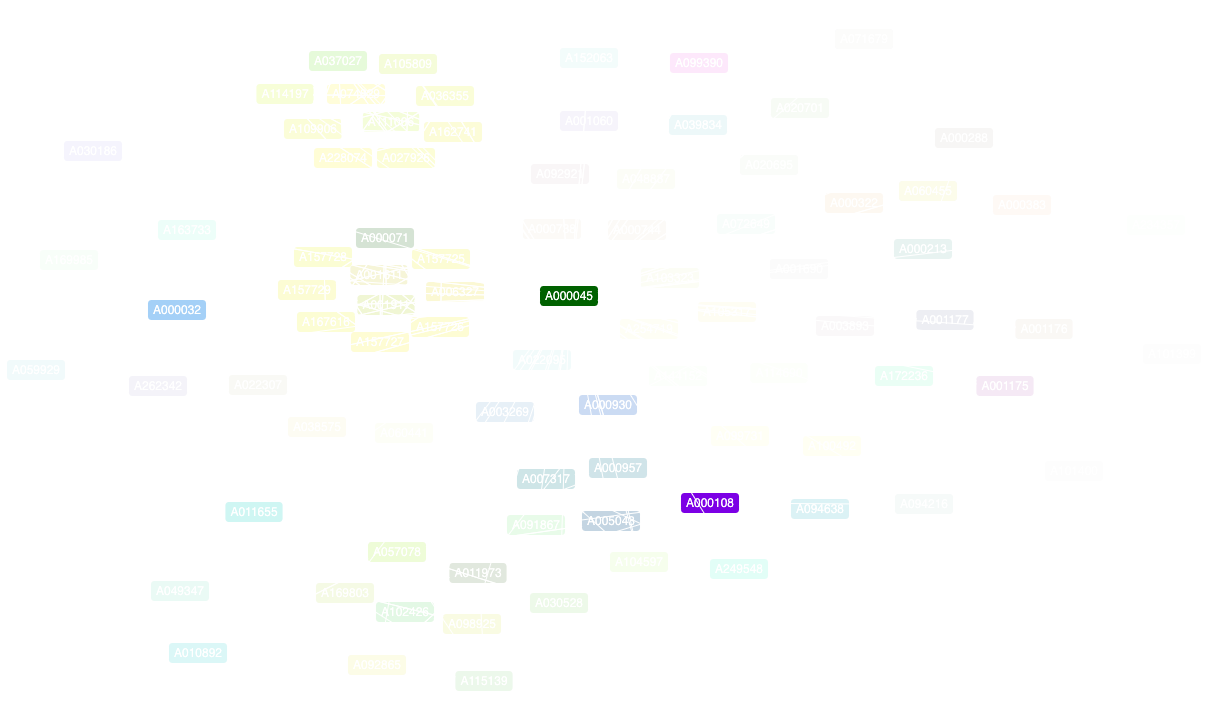
\includegraphics[width=12cm,height=8cm]{coloured}
\iffalse
\caption{Sequences network with labelel vertices, here we see that the sequence
of \textit{Fibonacci numbers} (\url{https://oeis.org/A000045}) and of
\textit{Catalan numbers} (\url{https://oeis.org/A000108}) are the two central
sequences, respectively.}
\fi
\end{figure}
\end{frame}


% Jordan Canonical Form {{{
\iffalse
\section{Jordan Canonical Forms}

\begin{frame}[fragile]
\frametitle{Jordan canonical form of a Riordan matrix}
\textit{Jordan canonical
form} of $A$ is defined by the relation $A\,X = X\, J$, where
\begin{displaymath}
X = \left[X_{1},\ldots,X_{\nu} \right]\in\mathbb{R}^{m\times m} \quad\text{and}\quad
J = \left[ \begin{array}{ccc}
    J_{1} \\
      & \ddots \\
      & & J_{\nu} \\
\end{array} \right] \in\mathbb{R}^{m\times m}
\end{displaymath}
for short $A\sim_{X}J$; in turn, those matrices depend on
\begin{displaymath}
X_{i}   = \left[\boldsymbol{x}_{i,1},\ldots,\boldsymbol{x}_{i,m_{i}} \right]\in\mathbb{R}^{m\times m_{i}}\quad\text{and}\quad
J_{i}   = \left[ \begin{array}{cccc}
    \lambda_{i} \\
    1 & \lambda_{i} \\
      & \ddots & \ddots \\
      & & 1 &\lambda_{i} \\
\end{array} \right] \in\mathbb{R}^{m_{i}\times m_{i}},
\end{displaymath}
for vectors $\boldsymbol{x}_{i,j} =
    Z_{i,2}^{j-1}\,Z_{i,1}\,\boldsymbol{v}$, $j\in\lbrace1,\ldots,m_{i}\rbrace$ and
    $i\in \lbrace 1,\ldots,\nu \rbrace$. Finally, $Z_{i,j} = \Phi_{i,j}(A)$
    are $A$'s \textit{component matrices}.
\vfill
\noindent\rule{\textwidth}{0.1pt}
{\footnotesize
Merlini \& Nocentini. \textit{Functions and Jordan Canonical Forms of Riordan
matrices}. \newline Linear Algebra and its Applications, under review.}
\end{frame}


\begin{frame}[fragile]
\frametitle{Jordan canonical form of a Riordan matrix}
\begin{theorem}
$ A \sim_{X} J \rightarrow g(A) \sim_{X} g(J) $
\end{theorem}
\begin{theorem}
$J_{i} = (\lambda_{i}+t,t)\rightarrow$ $f(J_{i})$ is a \emph{Toeplitz} matrix
\end{theorem}
\begin{displaymath}
\footnotesize
\hspace{-0.5cm}
J_{i}^{r} \boldsymbol{e}_{1}        = \left[\begin{matrix}\frac{{\left(r\right)}_{1} \lambda_{i}^{r}}{0!}\\\frac{{\left(r\right)}_{i}}{1!} \lambda_{i}^{r - 1}\\\frac{{\left(r\right)}_{2}}{2!} \lambda_{i}^{r - 2}\\\frac{{\left(r\right)}_{3}}{3!} \lambda_{i}^{r - 3}\\\frac{{\left(r\right)}_{4}}{4!} \lambda_{i}^{r - 4}\\\frac{{\left(r\right)}_{5}}{5!} \lambda_{i}^{r - 5}\\\frac{{\left(r\right)}_{6}}{6!} \lambda_{i}^{r - 6}\\\frac{{\left(r\right)}_{7}}{7!} \lambda_{i}^{r - 7}\end{matrix}\right],
\frac{\boldsymbol{e}_{1}}{J_{i}}    = \left[\begin{matrix}\frac{1}{\lambda_{i}}\\- \frac{1}{\lambda_{i}^{2}}\\\frac{1}{\lambda_{i}^{3}}\\- \frac{1}{\lambda_{i}^{4}}\\\frac{1}{\lambda_{i}^{5}}\\- \frac{1}{\lambda_{i}^{6}}\\\frac{1}{\lambda_{i}^{7}}\\- \frac{1}{\lambda_{i}^{8}}\end{matrix}\right],
\sqrt{J_{i}} \boldsymbol{e}_{1}     = \left[\begin{matrix}\sqrt{\lambda_{i}}\\\frac{1}{2 \sqrt{\lambda_{i}}}\\- \frac{1}{8 \lambda_{i}^{\frac{3}{2}}}\\\frac{1}{16 \lambda_{i}^{\frac{5}{2}}}\\- \frac{5}{128 \lambda_{i}^{\frac{7}{2}}}\\\frac{7}{256 \lambda_{i}^{\frac{9}{2}}}\\- \frac{21}{1024 \lambda_{i}^{\frac{11}{2}}}\\\frac{33}{2048 \lambda_{i}^{\frac{13}{2}}}\end{matrix}\right],

e^{J_{i} \alpha} \boldsymbol{e}_{1} = \left[\begin{matrix}e^{\alpha \lambda_{i}}\\\alpha e^{\alpha \lambda_{i}}\\\frac{\alpha^{2}}{2} e^{\alpha \lambda_{i}}\\\frac{\alpha^{3}}{6} e^{\alpha \lambda_{i}}\\\frac{\alpha^{4}}{24} e^{\alpha \lambda_{i}}\\\frac{\alpha^{5}}{120} e^{\alpha \lambda_{i}}\\\frac{\alpha^{6}}{720} e^{\alpha \lambda_{i}}\\\frac{\alpha^{7}}{5040} e^{\alpha \lambda_{i}}\end{matrix}\right],
log{\left (J_{i} \right )} \boldsymbol{e}_{1} = \left[\begin{matrix}\log{\left (\lambda_{i} \right )}\\\frac{1}{\lambda_{i}}\\- \frac{1}{2 \lambda_{i}^{2}}\\\frac{1}{3 \lambda_{i}^{3}}\\- \frac{1}{4 \lambda_{i}^{4}}\\\frac{1}{5 \lambda_{i}^{5}}\\- \frac{1}{6 \lambda_{i}^{6}}\\\frac{1}{7 \lambda_{i}^{7}}\end{matrix}\right]
\end{displaymath}
\vfill
\noindent\rule{\textwidth}{0.1pt}
{\footnotesize
Merlini \& Nocentini. \textit{Functions and Jordan Canonical Forms of Riordan
matrices}. \newline Linear Algebra and its Applications, under review.}
\end{frame}


\begin{frame}[fragile]
\frametitle{Jordan canonical form of a Riordan matrix}
Let $\mathcal{P}\sim_{X}J$, then Pascal's inverse can be computed by
$\mathcal{P}^{-1} = X\,J^{-1}\,X^{-1}$, where
\begin{displaymath}
X = \alpha_{0} \left[\begin{matrix}1 &  &  &  &  &  &  & \\0 & 1 &  &  &  &  &  & \\0 & 1 & 2 &  &  &  &  & \\0 & 1 & 6 & 6 &  &  &  & \\0 & 1 & 14 & 36 & 24 &  &  & \\0 & 1 & 30 & 150 & 240 & 120 &  & \\0 & 1 & 62 & 540 & 1560 & 1800 & 720 & \\0 & 1 & 126 & 1806 & 8400 & 16800 & 15120 & 5040\end{matrix}\right]\,
\end{displaymath}
depends on $\displaystyle\boldsymbol{v}= \left[\begin{matrix} \alpha_{0} & 0 &
0 & 0 & 0 & 0 & 0 & 0 \end{matrix}\right]$, $\alpha_{0}\in\mathbb{R}$.
\vfill
\noindent\rule{\textwidth}{0.1pt}
{\footnotesize
Merlini \& Nocentini. \textit{Functions and Jordan Canonical Forms of Riordan
matrices}. \newline Linear Algebra and its Applications, under review.}
\end{frame}

\begin{frame}[fragile]
\frametitle{Jordan canonical form of a Riordan matrix}
\begin{theorem}
$A\,X = X\,J$ and $B\,Y= Y\,J \rightarrow A \sim_{X\,Y^{-1}} B$. \\
Moreover, $f(A) \sim_{X\,Y^{-1}} f(B)$ also holds, for any
function $f$ defined on $\sigma(A)$.
\end{theorem}
Provided that $\mathcal{C}\sim_{Y}J$ and $\mathcal{P}\sim_{X}J$, then both
$\mathcal{P} \sim_{X\,Y^{-1}}\mathcal{C}$ and $\mathcal{C}
\sim_{Y\,X^{-1}}\mathcal{P}$ hold by
\begin{displaymath}
Y = \beta_{0} \left[\begin{matrix}1 &  &  &  &  &  &  & \\0 & 1 &  &  &  &  &  & \\0 & 2 & 2 &  &  &  &  & \\0 & 5 & 11 & 6 &  &  &  & \\0 & 14 & 52 & 62 & 24 &  &  & \\0 & 42 & 238 & 470 & 394 & 120 &  & \\0 & 132 & 1084 & 3176 & 4348 & 2844 & 720 & \\0 & 429 & 4956 & 20323 & 40562 & 42874 & 23148 & 5040\end{matrix}\right]
\end{displaymath}
which depends on $\displaystyle\boldsymbol{w}= \left[\begin{matrix} \beta_{0} &
0 & 0 & 0 & 0 & 0 & 0 & 0 \end{matrix}\right]$, $\beta_{0}\in\mathbb{R}$.
\vfill
\noindent\rule{\textwidth}{0.1pt}
{\footnotesize
Merlini \& Nocentini. \textit{Functions and Jordan Canonical Forms of Riordan
matrices}. \newline Linear Algebra and its Applications, under review.}
\end{frame}

\begin{frame}[fragile]
\frametitle{Jordan canonical form of the Fibonacci generator matrix}
Consider again the generator matrix $\mathcal{F}$ of Fibonacci numbers,
\begin{displaymath}
Z_{1,1} = \left[\begin{matrix}- \frac{\lambda_{2} - 1}{\lambda_{1} - \lambda_{2}} & \frac{1}{\lambda_{1} - \lambda_{2}}\\\frac{1}{\lambda_{1} - \lambda_{2}} & - \frac{\lambda_{2}}{\lambda_{1} - \lambda_{2}}\end{matrix}\right], \quad Z_{2,1} = \left[\begin{matrix}\frac{\lambda_{1} - 1}{\lambda_{1} - \lambda_{2}} & - \frac{1}{\lambda_{1} - \lambda_{2}}\\- \frac{1}{\lambda_{1} - \lambda_{2}} & \frac{\lambda_{1}}{\lambda_{1} - \lambda_{2}}\end{matrix}\right]
\end{displaymath}
\begin{displaymath}
\boldsymbol{x}_{1,1} = \left[\begin{matrix}- \frac{\left(\lambda_{2} - 1\right) \alpha_{0}}{\lambda_{1} - \lambda_{2}} + \frac{\alpha_{1}}{\lambda_{1} - \lambda_{2}}\\\frac{\alpha_{0}}{\lambda_{1} - \lambda_{2}} - \frac{\alpha_{1} \lambda_{2}}{\lambda_{1} - \lambda_{2}}\end{matrix}\right], \quad \boldsymbol{x}_{2,1} = \left[\begin{matrix}\frac{\left(\lambda_{1} - 1\right) \alpha_{0}}{\lambda_{1} - \lambda_{2}} - \frac{\alpha_{1}}{\lambda_{1} - \lambda_{2}}\\- \frac{\alpha_{0}}{\lambda_{1} - \lambda_{2}} + \frac{\alpha_{1} \lambda_{1}}{\lambda_{1} - \lambda_{2}}\end{matrix}\right]
\end{displaymath}
$\mathcal{F}X=XJ$ is the Jordan normal form of matrix $\mathcal{F}$, where
\begin{displaymath}
X = \left[\begin{matrix}- \frac{\left(\lambda_{2} - 1\right) \alpha_{0}}{\lambda_{1} - \lambda_{2}} + \frac{\alpha_{1}}{\lambda_{1} - \lambda_{2}} & \frac{\left(\lambda_{1} - 1\right) \alpha_{0}}{\lambda_{1} - \lambda_{2}} - \frac{\alpha_{1}}{\lambda_{1} - \lambda_{2}}\\\frac{\alpha_{0}}{\lambda_{1} - \lambda_{2}} - \frac{\alpha_{1} \lambda_{2}}{\lambda_{1} - \lambda_{2}} & - \frac{\alpha_{0}}{\lambda_{1} - \lambda_{2}} + \frac{\alpha_{1} \lambda_{1}}{\lambda_{1} - \lambda_{2}}\end{matrix}\right]
\quad\text{and}\quad J = \left[\begin{matrix}\lambda_{1} & 0\\0 & \lambda_{2}\end{matrix}\right].
\end{displaymath}
Let $\alpha_{0} = \alpha_{1} = 1$ in
$\displaystyle \mathcal{F}^{r} = \left(X\,J\,X^{-1}\right)^{r} = X\,J^{r}\,X^{-1}$, precisely
$$\mathcal{F}^{r}=\left[\begin{matrix}\frac{- \lambda_{2} + 2}{\lambda_{1} - \lambda_{2}} & \frac{\lambda_{1} - 2}{\lambda_{1} - \lambda_{2}}\\\frac{- \lambda_{2} + 1}{\lambda_{1} - \lambda_{2}} & \frac{\lambda_{1} - 1}{\lambda_{1} - \lambda_{2}}\end{matrix}\right]\,\left[\begin{matrix}\lambda_{1}^{r} & 0\\0 & \lambda_{2}^{r}\end{matrix}\right]\,\left[\begin{matrix}\frac{- \lambda_{2} + 2}{\lambda_{1} - \lambda_{2}} & \frac{\lambda_{1} - 2}{\lambda_{1} - \lambda_{2}}\\\frac{- \lambda_{2} + 1}{\lambda_{1} - \lambda_{2}} & \frac{\lambda_{1} - 1}{\lambda_{1} - \lambda_{2}}\end{matrix}\right]^{-1}.$$
\vfill
\noindent\rule{\textwidth}{0.1pt}
{\footnotesize
Merlini \& Nocentini. \textit{Functions and Jordan Canonical Forms of Riordan
matrices}. \newline Linear Algebra and its Applications, under review.}
\end{frame}

\fi
% }}}

\section{Co-recursion and relational programming}

\begin{frame}[fragile]
\frametitle{Riordan arrays are co-recursive data structures}

As in Haskell you write \mintinline{haskell}{let ones = 1 : ones :: [Int]}, in Scheme we write
\begin{minted}[baselinestretch=0.8]{scheme}
(define riordan-array
 (Λ (d h)
  (stream:dest/car+cdr (d ∅)
   ((dcar dcdr) (stream:cons
                 (list dcar)
                 ((stream:zip-with cons)
                  dcdr (riordan-array (series:× d h) h)))))))
\end{minted}

\begin{minted}[baselinestretch=0.8]{scheme}
(test '((1)
        (1 1)
        (1 2 1)
        (1 3 3 1)
        (1 4 6 4 1)
        (1 5 10 10 5 1)
        (1 6 15 20 15 6 1)
        (1 7 21 35 35 21 7 1)
        (1 8 28 56 70 56 28 8 1)
        (1 9 36 84 126 126 84 36 9 1))
 ((list○take 10) (riordan-array stream:1s stream:1s)))
\end{minted}
\end{frame}

\begin{frame}[fragile]
\frametitle{$\mu$Kanren for combinatorics}
\vfill
\begin{minted}[baselinestretch=0.8]{scheme}
(define fibonacciº
 (lambda (depth n α)
  (cond
   ((zero? depth) (≡ α (list n)))
   (else (fresh (β γ) (∧ (fibonacciº (sub1 depth) (sub1 n) β)
                         (fibonacciº (sub1 depth) (sub2 n) γ)
                         (appendº β γ α)))))))
\end{minted}
readily yields $\displaystyle f_{n} = \sum_{i=0}^{j}{{
{j}\choose{i} }\,f_{n-2\,j+i}}$ where
$\displaystyle j\leq \frac{n}{2}$.
\vfill
\begin{minted}[baselinestretch=0.8]{scheme}
(define tartagliaº
 (lambda (depth n k α)
  (cond
   ((zero? depth) (≡ α (list (list n k))))
   (else (fresh (β γ) (∧ (tartagliaº (sub1 depth) (sub1 n) (sub1 k) β)
                         (tartagliaº (sub1 depth) (sub1 n) k γ)
                         (appendº β γ α)))))))
\end{minted}
readily yields $\displaystyle { {p+m}\choose{r+m} } = \sum_{j=0}^{m-1}{{
{m-1}\choose{j} }{ {p-1+m}\choose{r-j+m} }}$ for $p,r,m\in\mathbb{N}$.

\end{frame}

\begin{frame}[fragile]
\frametitle{Kanren-light for certified logic programming}
Kanren-light extends the HOL-light's tactics mechanism with 
\begin{itemize}
\item explicit use of meta-variables, 
\item backtracking during the proof search and
\item a layer of tools to interface with the underlying proof process
\end{itemize}

\begin{minted}[baselinestretch=0.8]{ocaml}
# list_of_stream
    (solve APPEND_SLV
           `??x y. APPEND x y = [1;2;3]`);;

val it : (term list * thm) list =
  [([`x = []`; `y = [1; 2; 3]`],
    |- APPEND [] [1; 2; 3] = [1; 2; 3]);
   ([`x = [1]`; `y = [2; 3]`],
    |- APPEND [1] [2; 3] = [1; 2; 3]);
   ([`x = [1; 2]`; `y = [3]`],
    |- APPEND [1; 2] [3] = [1; 2; 3]);
   ([`x = [1; 2; 3]`; `y = []`],
    |- APPEND [1; 2; 3] [] = [1; 2; 3])]
\end{minted}
\end{frame}

\begin{frame}[fragile]
\frametitle{Kanren-light for certified logic programming}
\begin{minted}[baselinestretch=0.8]{ocaml}
let sexp_INDUCT,sexp_RECUR = define_type
  "sexp = Symbol string
        | List (sexp list)";;
\end{minted}
\vfill
\begin{minted}[baselinestretch=0.8]{ocaml}
let EVAL_RULES,EVAL_INDUCT,EVAL_CASES = new_inductive_definition
  `(!e q. EVAL e (List [Symbol "quote"; q]) q) /\
   (!e a x. RELASSOC a e x ==> EVAL e (Symbol a) x) /\
   (!e l. EVAL e (List (CONS (Symbol "lambda") l))
                 (List (CONS (Symbol "lambda") l))) /\
   (!e l l'. ALL2 (EVAL e) l l'
             ==> EVAL e (List (CONS (Symbol "list") l)) (List l')) /\
   (!e f x x' v b y.
      EVAL e f (List [Symbol "lambda"; List[Symbol v]; b]) /\
      EVAL e x x' /\ EVAL (CONS (x',v) e) b y
      ==> EVAL e (List [f; x]) y)`;;
\end{minted}
\vfill
\begin{minted}[baselinestretch=0.8]{ocaml}
let [_; i2,s2] = take 2 (solve EVAL_SLV `??q. EVAL [] q q`);;

# vsubst [`"x"`,hd (frees (rand (hd i2)))] (hd i2);;
val it : term = 
    `q = '((lambda (x) (list x x)) (lambda (x) (list x x)))`
\end{minted}
\end{frame}

\section{On GitHub}

\begin{frame}[fragile]
\frametitle{The repos behind this work}
\url{https://github.com/massimo-nocentini/PhD-thesis}
\vfill
\url{https://github.com/massimo-nocentini/on-scheme}
\vfill
\url{https://github.com/massimo-nocentini/on-python}
\vfill
\url{https://github.com/massimo-nocentini/oeis-tools}
\vfill
\url{https://github.com/massimo-nocentini/simulation-methods}
\vfill
\url{https://github.com/massimo-nocentini/learning-haskell}
\vfill
\url{https://github.com/massimo-nocentini/kanren-light}
\vfill
\url{https://github.com/massimo-nocentini/recurrences-unfolding}
\vfill
\url{https://github.com/massimo-nocentini/microkanrenpy}
\vfill
\url{https://github.com/massimo-nocentini/reasoning-about-little-books}
\end{frame}

\section{Thanks}

\iffalse
\begin{frame}{ }
\Huge Thanks!
\end{frame}
\fi

\end{document}

